\chapter{Introduction}
\label{ch:introduction}
Modern Operational Technology (OT) such as Industrial Control Systems (ICS) increasingly rely on Information and Communication Technology (ICT) for monitoring and control~\cite{Stouffer2023}.
As a consequence, the resemblance of OT and Information Technology (IT) systems increases, as OT systems adopt IT technology.
This development leads to new possibilities including the integration of distributed OT into Supervisory Control And Data Acquisition (SCADA) systems.
Nevertheless, new challenges arise from the increased usage of ICT in OT systems.

According to \citeauthor{Stouffer2023} \cite{Stouffer2023}, the typical long life cycle of OT systems and their unique requirements regarding performance, reliability, security, safety, privacy, and environmental impact have to be taken into account when designing, operating, and maintaining OT systems.
In the following, we focus on the information security of OT systems.
Although a variety of information security solutions exist for IT, migration of existing approaches to the OT domain may not be a viable solution due to the differing system characteristics, risks, and priorities.
An example for the differing priorities are information confidentiality and access control.
While the prevention of unauthorized access represents the core objective of IT security approaches, OT systems and especially OT-based critical infrastructure prioritize system availability and reliability.

In the energy-related sector, the infrastructure currently transforms from traditional top-down energy transmission and distribution systems to so-called smart grids with bidirectional data and energy flow \cite{Fang2012}.
In contrast to traditional energy grids, smart grids are adaptive, self-monitoring and self-healing infrastructures that enable pervasive control and monitoring of distributed heterogeneous grid participants.
As illustrated in \autoref{fig:smart_grid_overview}, a smart grid interconnects not only producers, consumers, and control centers, but also integrates prosumers, substations, and other grid-related elements.
The distribution of formerly centralized entities, such as power plants and control centers, necessitates not only changes in energy infrastructure but also leads to an increased reliance on communication solutions.
\begin{figure}
    \centering
    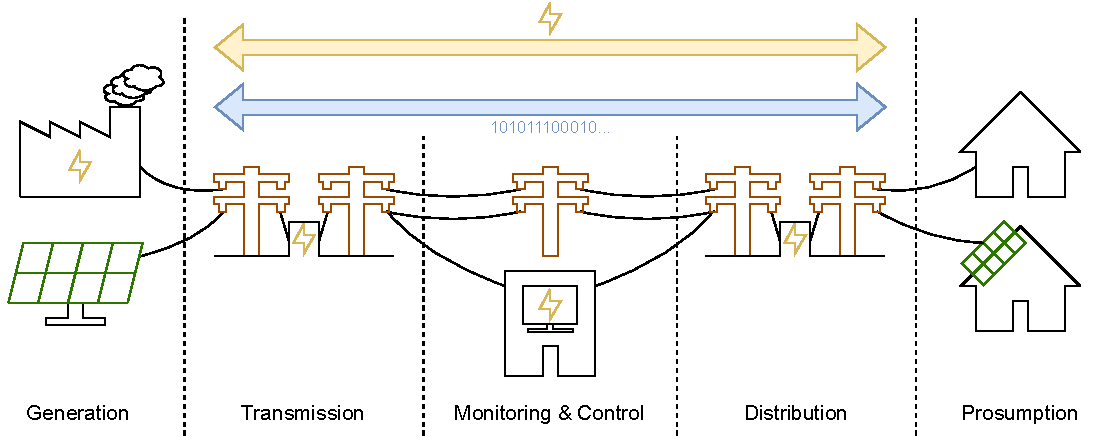
\includegraphics[width=.9\linewidth]{figures/smart_grid_overview_extended_color.drawio.pdf}
    \caption{Bidirectional power and data distribution in a smart electricity grid.}
    \label{fig:smart_grid_overview}
\end{figure}

The IEC 61850 series provides standards for the communication networks of digital energy systems~\cite{IEC61850P5}.
The goals of the IEC 61850 series are seamless communication and interoperability of systems in a smart energy grid.
Although standards for the communication of digital energy systems are provided by the IEC 61850, information security is not an objective of these standards.
To overcome this problem, the IEC 62351 standard series was created by the~\citeauthor{IEC62351P6}.
Part 6 of the IEC 62351 series provides standardized security means for communication compliant to IEC 61850~\cite{IEC62351P6}.
Moreover, Part 8 of the IEC 62351 series provides a role-based access control concept for power systems~\cite{IEC62351P8}.

The focus of this thesis is on the communication aspects of smart grids.
To enhance the communication security and overcome the limitations of existing standards, we propose an approach that can be integrated into smart electricity grids.
The field of application of the approach proposed in this thesis is known as a Substation Automation System (SAS).
A SAS represents the entirety of communication and control equipment of a substation~\cite{Padilla2015}.
A substation is a facility of a high-voltage electricity grid connecting power transmission and distribution lines that use different voltage levels~\cite{oshaSubstation}.
A substation and its SAS represent a specific type of ICS.
The tasks of a SAS are time-critical and have to be executed reliably, as the electricity sector and its substations are critical infrastructures.

\section{Objective}
\label{sec:introduction:objective}
Although standards regarding the communication networks of smart grid systems are widely accepted and utilized, information security continues to confront unresolved challenges.
Historical evidence indicates that economically or politically motivated adversaries pose a risk to OT systems, including energy-related systems.
The \citeauthor{canada2021} \cite{canada2021} published a list of 28 OT-related cybersecurity incidents between 2010 and 2020, including incidents in energy-related sectors.
These incidents comprise 13 state-sponsored incidents, 13 cybercrime incidents, and two incidents perpetrated by thrill-seeking individuals.
The state-sponsored incidents include the Stuxnet malware deployed in Iranian nuclear power and enrichment facilities in 2010 \cite{bbc2010}, the Shamoon malware used against Saudi Aramco in 2012 \cite{reuters2012}, the Blackenergy malware used to attack Ukrainian power distribution systems in 2015 \cite{cisa2021a}, the Industroyer/CrashOverride malware used to shut down remote terminal units of a Ukrainian power transmission facility in 2016 \cite{reuters2016,cisa2021b}, and the Triton/Trisis malware used to attack Triconex Safety Instrumented System (SIS) controllers in 2017 \cite{johnson2017}.
% ...and other incidents in 2013, 2014, 2015, 2017, 2018 as well as 2020 \cite{wsj2015,cisa2018a,bsi2014,hdn2017,vice2017,cisa2018b,toi2020,warrick2020}.

Despite the existence of standards for communication and information security including the IEC 61850 and 62351, there are remaining challenges in order to secure SAS communication.
This thesis focuses on these remaining challenges to enhance the information security of SAS communication.
As stated by \citeauthor{Ishchenko2018} \cite{Ishchenko2018}, these challenges include, among others, ensuring the integrity and authenticity of substation control and protection communication without compromising the time criticality.
For this purpose, cryptographic signature and verification approaches can be employed in the SAS environment.
According to \citeauthor{Elbez2019} \cite{Elbez2019}, the strict time constraints of the low latency communication in substations are key factors for the information security.
Accordingly, Public Key Cryptography (PKC), which was formerly specified by the IEC 62351 standards, seemed to be inappropriate due to computational complexity and latency.

% Based on this proposed approach, the following research questions are going to be answered in the course of this thesis:
Due to an increase in processing performance of IT and OT devices nowadays, this thesis examines the applicability of effective and efficient PKC in substations.
For this purpose, this thesis proposes new cryptographic and cybersecurity approaches for authentication, authorization, and access control.
Moreover, the thesis discusses the employment of speedup techniques to enable the usage of secure PKC in time-critical OT systems.
Therefore, the following research questions are going to be answered in the course of this thesis:
\begin{description}
    \item[RQ1] How can expressive and flexible yet computationally expensive access control approaches such as Attribute-Based Access Control (ABAC) be employed to enable prevention of unauthorized access, enable the Separation of Duties (SoD), and ensure the Principle of Least Privilege (PoLP) in a time-critical SAS environment?
    \item[RQ2] How can a secure and lightweight PKC approach be designed and implemented, that is able to ensure the authenticity, integrity, and non-repudiation of communication in a time-critical SAS environment?
    \item[RQ3] How can authentication, authorization, and access control be integrated into a malleable, scalable, and lightweight cryptosystem for time-critical SAS communication?
\end{description}

\section{Contribution}
\label{sec:introduction:contribution}
With the aim of providing means to enhance the information security in a SAS, we propose a \textbf{C}ertificateless \textbf{A}ttribute-Based \textbf{S}erver-Aided \textbf{C}ryptosystem for \textbf{S}ubstation \textbf{A}utomation \textbf{S}ystems (CASC-SAS).
The main objective of the proposed approach is to provide secure protocols, algorithms, and schemes for SAS communication.
The provided protocols, algorithms, and schemes aim to satisfy SAS security requirements such as integrity, authenticity, access control, and non-repudiation.
Furthermore, the approach takes the specific characteristics, risks, and priorities of OT, ICS, and SAS into account.
To address the aforementioned objectives and considerations, this thesis comprises the following contributions:
\begin{itemize}
    \item Identification of security, safety, availability, performance, and compatibility requirements of the proposed approach, and development of a system model, which represents the corresponding field of application.
    \item Design of a server-aided attribute-based authorization and access control approach, which relies on speedup techniques such as access decision caching and policy evaluation precomputation.
    \item Design of a certificateless attribute-based server-aided authentication approach, which provides algorithm-agnostic cryptographic protocols and services as well as an AB-PKC signature scheme.
    \item Design of a certificateless attribute-based server-aided cryptosystem for SAS, which integrates authentication, authorization, and access control into a dual-path four-layered system architecture.
    \item Implementation of the proposed approach using high-level programming languages, and deployment of the implementation to a test bed that mimics the behavior of an interconnected OT system.
    \item Security evaluation to prove the security characteristics of the approach.
    \item Performance evaluation to demonstrate the applicability of the approach in an OT environment with strict time and resource constraints.
    \item Compatibility evaluation to demonstrate the feasibility of the approach for the construction and retrofitting of a SAS.
\end{itemize}

\section{Structure}
\label{sec:introduction:structure}
The following section presents the structure of this thesis.
The structure consists of six chapters and is illustrated in \autoref{fig:thesis_structure}.

\Cref{ch:introduction} serves to motivate communication security in OT and SAS.
In addition, the chapter presents the research questions and outlines the objective and contributions of the proposed approach.

\Cref{ch:fundamentals} presents the fundamental concepts upon which this thesis and its proposed approach are based.
Among other concepts, it introduces the fundamentals of OT, ICS, information security, system safety, access control, and cryptography.

\Cref{ch:relatedwork} presents a review of the existing literature and offers a delineation between the literature and the proposed approach.

\Cref{ch:approach} defines the proposed SAS security approach, including its system model, requirements, potential adversarial attacks, security policies, security architecture, and realization.
Furthermore, this chapter elucidates the components, algorithms, schemes, and protocols of the proposed security approach.

\Cref{ch:evaluation} presents a comprehensive evaluation of the proposed approach, encompassing security, performance, and compatibility considerations.
Furthermore, the chapter discusses the results of the evaluation, contextualizes the approach within the existing literature by comparing it to related approaches, and describes the limitations and constraints inherent to the evaluation and proposed approach.

In conclusion, \cref{ch:conclusion} provides insight into prospective future research and presents a summary of the thesis.
\begin{figure}
    \centering
    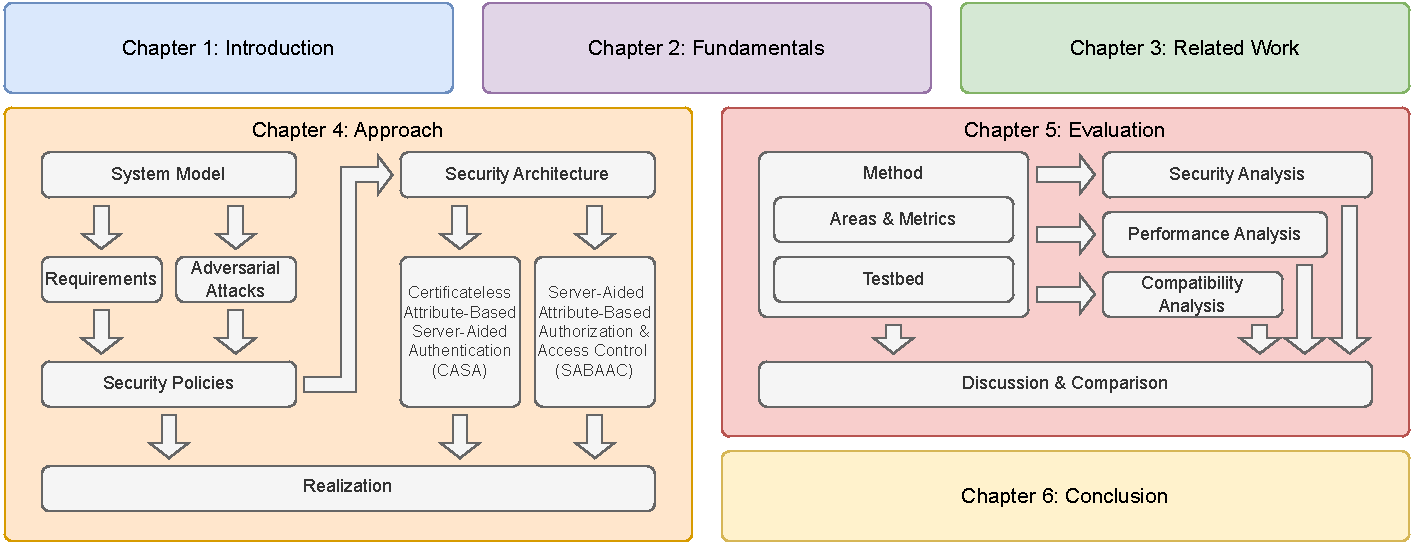
\includegraphics[width=1.\linewidth]{figures/thesis_structure.drawio.pdf}
    \caption{Structure of the thesis consisting of six interrelated chapters.}
    \label{fig:thesis_structure}
\end{figure}
